\documentclass[11pt]{article}

\usepackage[T1]{fontenc}
\usepackage{geometry}
\usepackage{amsmath, amssymb, amsthm}
\usepackage{listings}
% \usepackage{courier}
\usepackage{xcolor}
\usepackage{graphicx}
\usepackage{fancyhdr}
\usepackage{lipsum}
% \usepackage{subfigure}
\usepackage{caption}
\usepackage{subcaption}
\usepackage{float}
\usepackage{hyperref}

\makeatletter
\renewcommand\@biblabel[1]{}
\renewenvironment{thebibliography}[1]
     {\section*{\refname}%
      \@mkboth{\MakeUppercase\refname}{\MakeUppercase\refname}%
      \list{}%
           {\leftmargin0pt
            \@openbib@code
            \usecounter{enumiv}}%
      \sloppy
      \clubpenalty4000
      \@clubpenalty \clubpenalty
      \widowpenalty4000%
      \sfcode`\.\@m}
     {\def\@noitemerr
       {\@latex@warning{Empty `thebibliography' environment}}%
      \endlist}
\makeatother

% \captionsetup[table]{skip=10pt}

\geometry{a4paper, margin=1in, headheight=14pt}

\pagestyle{fancy}
\renewcommand\headrulewidth{0.4pt}
\fancyhead[L]{\scshape Experiment VI}
% \lhead{Experiment I}
\rhead{}
\cfoot{\thepage}

\definecolor{darkgreen}{rgb}{0.2, 0.6, 0.4}
\definecolor{darkblue}{rgb}{0.2, 0.4, 0.8}
\lstset{ 
  basicstyle=\footnotesize\ttfamily,
  commentstyle=\color{gray},
  % extendedchars=true,
  % keepspaces=true,
  keywordstyle=\color{darkblue},
  % numbers=left,
  % numbersep=5pt,
  % numberstyle=\tiny\color{gray},
  stringstyle=\color{darkgreen},
  tabsize=4,
  % frame=lines,
  aboveskip=2em,
  belowskip=2em,
  breaklines=true
}

\newcommand\pp[2]{\frac{\partial #1}{\partial #2}}
\newcommand\E[1]{\langle #1 \rangle}

\title{
        \Large\textsc{PH2103: Physics Laboratory III} \\
        \vspace{10pt}
        \Huge \textbf{Polarization of light} \\
        \vspace{5pt}
        \large{Polarisers and waveplates, Malus Law.}
}
\author{
        \large Satvik Saha%
        \thanks{Email: \tt ss19ms154@iiserkol.ac.in}
        \\\textsc{\small 19MS154}
}
\date{\normalsize
        \textit{Indian Institute of Science Education and Research, Kolkata, \\
        Mohanpur, West Bengal, 741246, India.} \\
        \vspace{10pt}
        \today
}

\begin{document}
        \maketitle

        % \renewcommand{\abstractname}{Aims}
        \begin{abstract}
                In this experiment, we verify the Malus Law of polarization and study the effect of polarisers and waveplates on the intensity
                of light.
        \end{abstract}

        \section{Theory}
        We have seen in our discussion of Lissajous figures that the superposition of two orthogonal vectors, whose amplitudes vary sinusoidally
        with the same frequency but with some phase difference, produces a new vector whose tip traces an ellipse.
        In other words, consider the parametric curve described by
        \[
                x(t) = A\cos(\omega t), \qquad y(t) = B\cos(\omega t + \phi).
        \]
        Eliminating the parameter $t$ gives
        \[
                \frac{x^2}{A^2} + \frac{y^2}{B^2} - \frac{2xy}{AB}\cos\phi = \sin^2\phi.
        \]
        Conversely, any light wave polarized as such (elliptically, which includes circular and linear\footnote{A line is simply a degenerate ellipse})
        can be decomposed into two sinusoidal components along any two perpendicular axes.
        A \textit{polariser} functions by removing the component along one of its axes and allowing the remainder to pass.
        A \textit{waveplate} functions by introducing an additional phase difference between the components along its axes 
        (informally called the fast and slow axes).
        
        \paragraph{Polarisers}
        Consider a polariser whose transmission axis is inclined at an angle $\theta$ with respect to the oscillation of a linearly polarised wave.
        If this wave is of the form $E(t) = E_0\cos{\omega t}$, note that its intensity is given by
        \[
                I_0 = \epsilon_0 c \langle E^2 \rangle = \frac{1}{2}\epsilon_0 c E_0^2.
        \]
        At any moment, the electric field vector can be decomposed into components along the transmission axis, and perpendicular to the transmission
        axis.
        \[
                E_\parallel(t) = E_0\cos{\omega t}\cos\theta, \qquad E_\perp(t) = E_0\cos{\omega t}\sin\theta.
        \]
        When passing through the polariser, only $E_\parallel$ survives. Its intensity is simply
        \[
                I = \epsilon_0 c \langle E_\parallel^2 \rangle = \frac{1}{2}\epsilon_0 c E_0^2\cos^2\theta.
        \]
        Thus, we have obtained a relation between the initial and final intensities. This is called the Malus Law.
        \[
                I = I_0 \cos^2\theta.
        \]
        Of course, this holds only for linearly polarised light. If instead we start with circularly polarized light, the components
        along and perpendicular to the transmission axis will always have the same amplitude, regardless of the orientation of the polariser\footnote{
                In all these cases, we of course assume that the polariser/waveplate is normal to the direction of propagation of the waves.
        }
        (this is a simple consequence of symmetry). Thus, the component passing through must have exactly half the intensity of the original light,
        so $I = I_0 /2$.

        An analogous argument can be used for unpolarised light. Different waves in the incoming beam have their electric fields oscillating
        in different, random orientations. Thus, we can approximate $\theta$ as a random variable which varies uniformly over $[0, 2\pi]$.
        The average of $\cos^2\theta$ is thus $\langle\cos^2\theta\rangle = 1 /2$, so the transmitted intensities of all these waves
        adds up to $I_0 /2$, half of the incoming intensity.

        \paragraph{Waveplates}
        A waveplate comprises of an anisotropic medium which exhibits different refractive indices along its fast and slow axes. If
        light passes perpendicular to both these axes over a thickness $t$, the components along the fast and slow axes accumulate a
        path difference $d = t\Delta n$, where $\Delta n$ is the difference in the fast and slow refractive indices.
        This corresponds to a phase difference of $\delta = 2\pi t\Delta n / \lambda$.

        Suppose a waveplate imparts a phase difference of $\delta$ between components along its fast and slow axis. Thus, a linearly polarised
        wave striking the waveplate at an angle $\theta$ has components as described earlier. We add a phase $\delta$ to one of them to obtain
        \[
                E_\parallel(t) = E_0\cos(\omega t)\cos\theta, \qquad E_\perp(t) = E_0\cos(\omega t + \delta)\sin\theta.
        \]
        Thus, the waveplate changes the nature of the elliptic polarisation. Note that the intensity of the outgoing beam,
        which is equal to the sum of intensities of both outgoing components, remains unaltered.
        \[
                I = I_\parallel + I_\perp = \frac{1}{2}\epsilon_0c(E_0\cos^2\theta + E_0\sin^2\theta) = \frac{1}{2}\epsilon_0cE_0^2 = I_0.
        \]
        In the special case that $\theta = \pi /4$ and $\delta = \pi /2$, note that
        \[
                E_\parallel(t) = \frac{1}{\sqrt{2}}E_0\cos(\omega t), \qquad E_\perp(t) = -\frac{1}{\sqrt{2}}E_0\sin(\omega t).
        \]
        Thus, we have converted linearly polarised light into circularly polarised light.
        We can clearly see that $I_\parallel = I_\perp = I_0 / 2$. The principle of reversibility shows that
        we can also convert circularly polarised light into linearly polarised light by running this system backwards.
        This particular waveplate is called a \textit{quarter waveplate}, because it imparts a path difference of $\lambda /4$. \\

        In the special case that $\delta = \pi$, note that
        \[
                E_\parallel(t) = E_0\cos(\omega t)\cos\theta, \qquad E_\perp(t) = -E_0\cos(\omega t)\sin\theta.
        \]
        Thus, the linearly polarized light remains linear, but has been reflected about the parallel component, i.e.\ deflected by an angle
        $2\theta$. This particular waveplate is called a \textit{half waveplate}, because it imparts a path difference of $\lambda /2$. \\

        In any case, note that when the incoming linearly polarised beam is directed along one of the axes, i.e.\ one of $E_\parallel$ 
        and $E_\perp$ is zero, the waveplate has no effect. Otherwise, the waveplate has the effect of distributing the intensity
        of the beam over both axes. This can be checked by removing one of the components using a polariser.
        Additionally, a polariser has no effect on a linearly polarised beam only when their axes are aligned too (\theta = 0 in the Malus Law).
        Thus, such a waveplate-polariser system will produce a full intensity outgoing beam only when all of their axes
        (oscillation of the electric field, fast/slow axis of the waveplate, transmission axis of the polariser) are aligned.

        \paragraph{Imperfect polarisers}
        Suppose that the polarisers used are imperfect, such that the transmission axis allows a fraction $\beta \approx 1$ of the electric field
        amplitude to pass and the perpendicular axis allows a fraction $\alpha \approx 0$ of the electric field amplitude.
        Linearly polarised light striking this polariser such that its polarisation angle is inclined by $\theta$ with the transmission axis
        will thus transform into
        \[
                E_\parallel = \beta E_0\cos(\omega t)\cos\theta, \qquad E_\perp = \alpha E_0\cos(\omega t)\sin\theta.
        \]
        The intensity distribution is of the form
        \[
                I(\theta) = \frac{1}{2}\epsilon_0E_0^2(\beta^2\cos^2\theta + \alpha^2\sin^2\theta) = I_0 (\alpha^2 + (\beta^2 - \alpha^2)\cos^2\theta).
        \]
        Note that $I_{max} = \beta^2I_0$ and $I_{min} = \alpha^2 I_0$. The quantity
        \[
                \mathcal{P} = \frac{I_{max} - I_{min}}{I_{max} + I_{min}} = \frac{\beta^2 - \alpha^2}{\beta^2 + \alpha^2}
        \]
        is called the degree of polarisation. Comparing the distribution with the curve $a + b\cos^2(x - c)$, we note that
        $I_0\alpha^2 = a$ and $I_0(\beta^2 - \alpha^2) = b$, so $\mathcal{P} = b / (2a + b)$.

        With a slightly different definition of the degree of polarisation, we may write
        \[
                \mathcal{P}' = 1 - \frac{I_{min}}{I_{max}} = 1 - \frac{\alpha^2}{\beta^2} = \frac{b}{a + b}.
        \]

        Suppose instead that we start with elliptically polarised light of the form $E_x = A\cos(\omega t)$, $E_y = B\sin(\omega t)$\footnote{
                It is always possible to choose appropriate axes to resolve the components this way. Specifically, any ellipse has this parametrization
                along the major and minor axes.
        }.
        We see that
        \[
                I_0 = \frac{1}{2}\epsilon_0 c (A^2 + B^2) = \frac{1}{2}\epsilon_0 c E_0^2.
        \]
        Rotating the frame by $\theta$ and scaling by $\beta$ and $\alpha$, we see that
        \[
                E_\parallel = \beta\left(A\cos\theta\cos(\omega t) - B\sin\theta\sin(\omega t)\right), \qquad
                E_\perp     = \alpha\left(A\sin\theta\cos(\omega t) + B\cos\theta\sin(\omega t)\right).
        \]
        The intensity distribution is thus of the form
        \[
                I(\theta) = \epsilon_0 c \left\langle\beta^2(A\cos\theta\cos(\omega t) - B\sin\theta\sin(\omega t))^2 + 
                        \alpha^2(A\sin\theta\cos(\omega t) + B\cos\theta\sin(\omega t))^2\right\rangle.
        \]
        Note that
        \begin{align*}
                \langle (A\cos\theta\cos(\omega t) - B\sin\theta\sin(\omega t))^2 \rangle = \frac{1}{2}A^2\cos^2\theta + \frac{1}{2}B^2\sin^2\theta, \\
                \langle (A\sin\theta\cos(\omega t) + B\cos\theta\sin(\omega t))^2 \rangle = \frac{1}{2}A^2\sin^2\theta + \frac{1}{2}B^2\cos^2\theta.
        \end{align*}
        This is because the cross terms $\langle \cos(\omega t)\sin(\omega t) \rangle = 0$. 
        Thus,
        \[
                I(\theta) = \frac{1}{2}\epsilon_0 c \left[(\beta^2 A^2 + \alpha^2 B^2)\cos^2\theta + (\beta^2B^2 + \alpha^2A^2)\sin^2\theta\right].
        \]
        With an appropriate choice of constants, this again simplifies to the form
        \[
                I(\theta) = a + b\cos^2\theta.
        \]
        
        \section{Experimental setup}
        Light from a diode laser is passed through a polariser, which is oriented so as to obtain linearly polarised light of the maximum possible
        intensity. Once this adjustment is made, the light is passed through another polariser (an analyser).
        The analyser is rotated and the resultant intensity is measured as a function of this rotation angle. \\

        Now, rotate the analyser so that the transmitted intensity is minimum. This must be the crossed position, where the transmission axes
        of the polariser and analyser are perpendicular. Insert a quarter waveplate between them, and rotate it such that the transmitted intensity
        is minimum once again. In this orientation, for the waveplate to have had no effect, we deduce that the waveplate anisotropy axes
        are aligned with the transmission axes of the polarisers. Rotate the waveplate by $\pi /4$. It must now produce circularly polarised light,
        which can be verified by rotating the analyser; very little variation in intensity should be observed.
        Any such variation is the result of the ellipticity of the light, and the ratio of maximum and minimum observed intensities is a measure of this.

        % If the same is repeated with a half waveplate, we know that after the $\pi/4$ rotation, the transmitted light must be linearly polarised
        % and perpendicular to the incoming light, which makes it polarised directly along the transmission axis of the (crossed) analyser.
        % This can be verified by noting that the overall transmitted intensity is maximum at this position upon rotation.
        
        \section{Experimental data and analysis}
        
        \subsection{Processing and plotting}
        All data has been gathered into an Excel spreadsheet, read using \texttt{pandas} and processed using \texttt{numpy}.
        The code used has been listed below.
        
        \lstinputlisting[language=Python]{plot.py}

        \begin{figure}[H]
        \begin{subfigure}[b]{0.50\textwidth}
                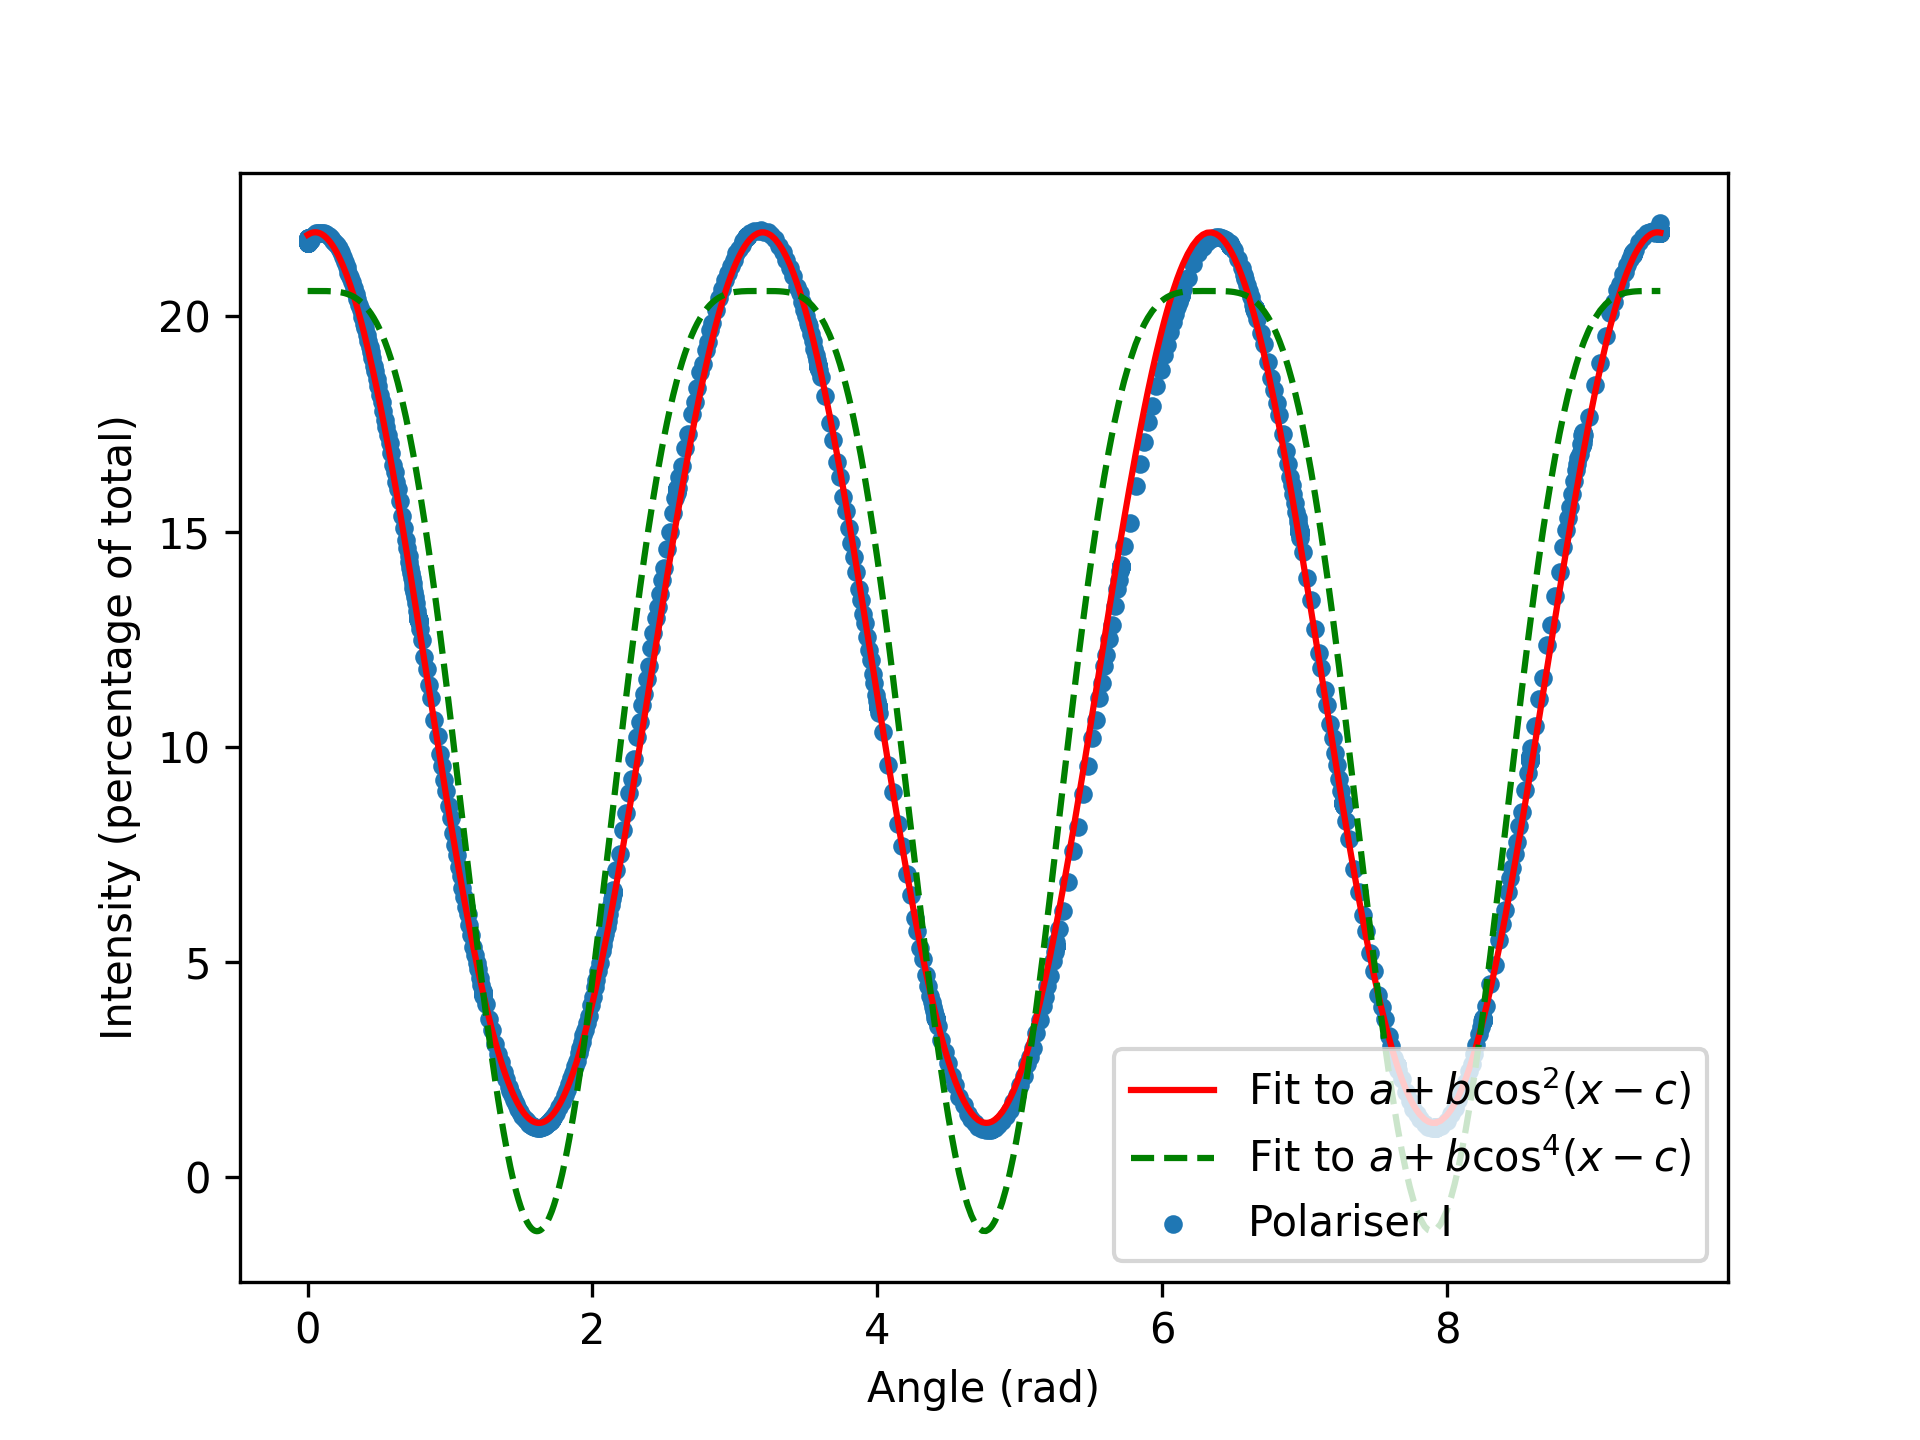
\includegraphics[width=1.1\textwidth]{./pol_1.png}
                \caption{Polariser I}
        \end{subfigure}
        \begin{subfigure}[b]{0.50\textwidth}
                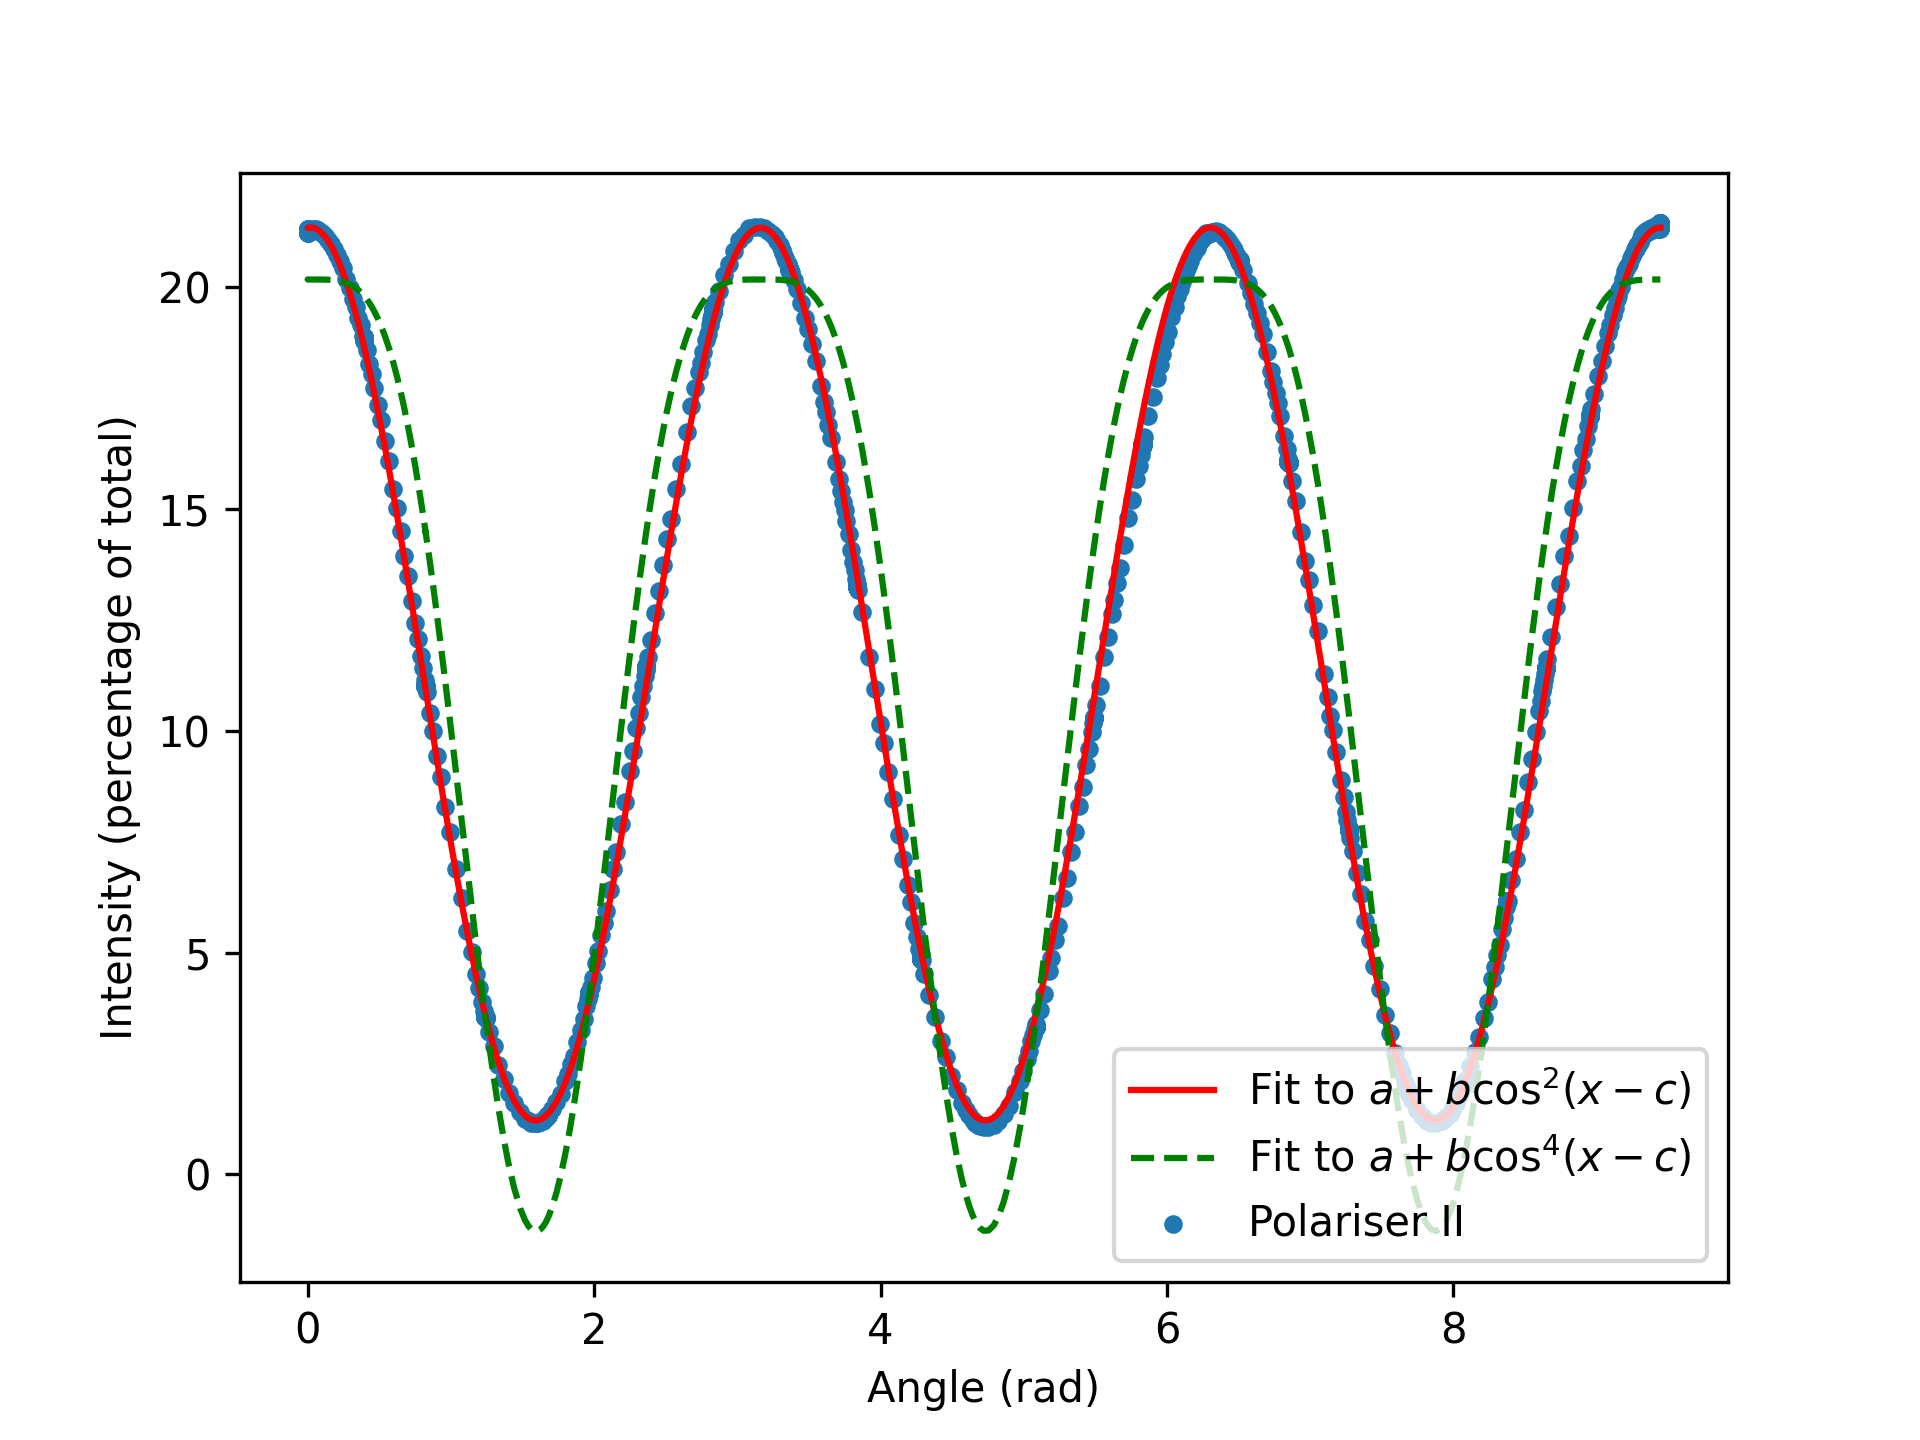
\includegraphics[width=1.1\textwidth]{./pol_2.png}
                \caption{Polariser II}
        \end{subfigure}
        \caption{Intensities from the polariser-analyser setup as a function of the rotation angle. Note that the fit against $a + b\cos^2(x - c)$
        is almost perfect, while the $a + b\cos^4(x - c)$ curve does not fit at all.}
        \label{fig:polarisers}
        \end{figure}

        \begin{figure}[H]
        \begin{subfigure}[b]{0.50\textwidth}
                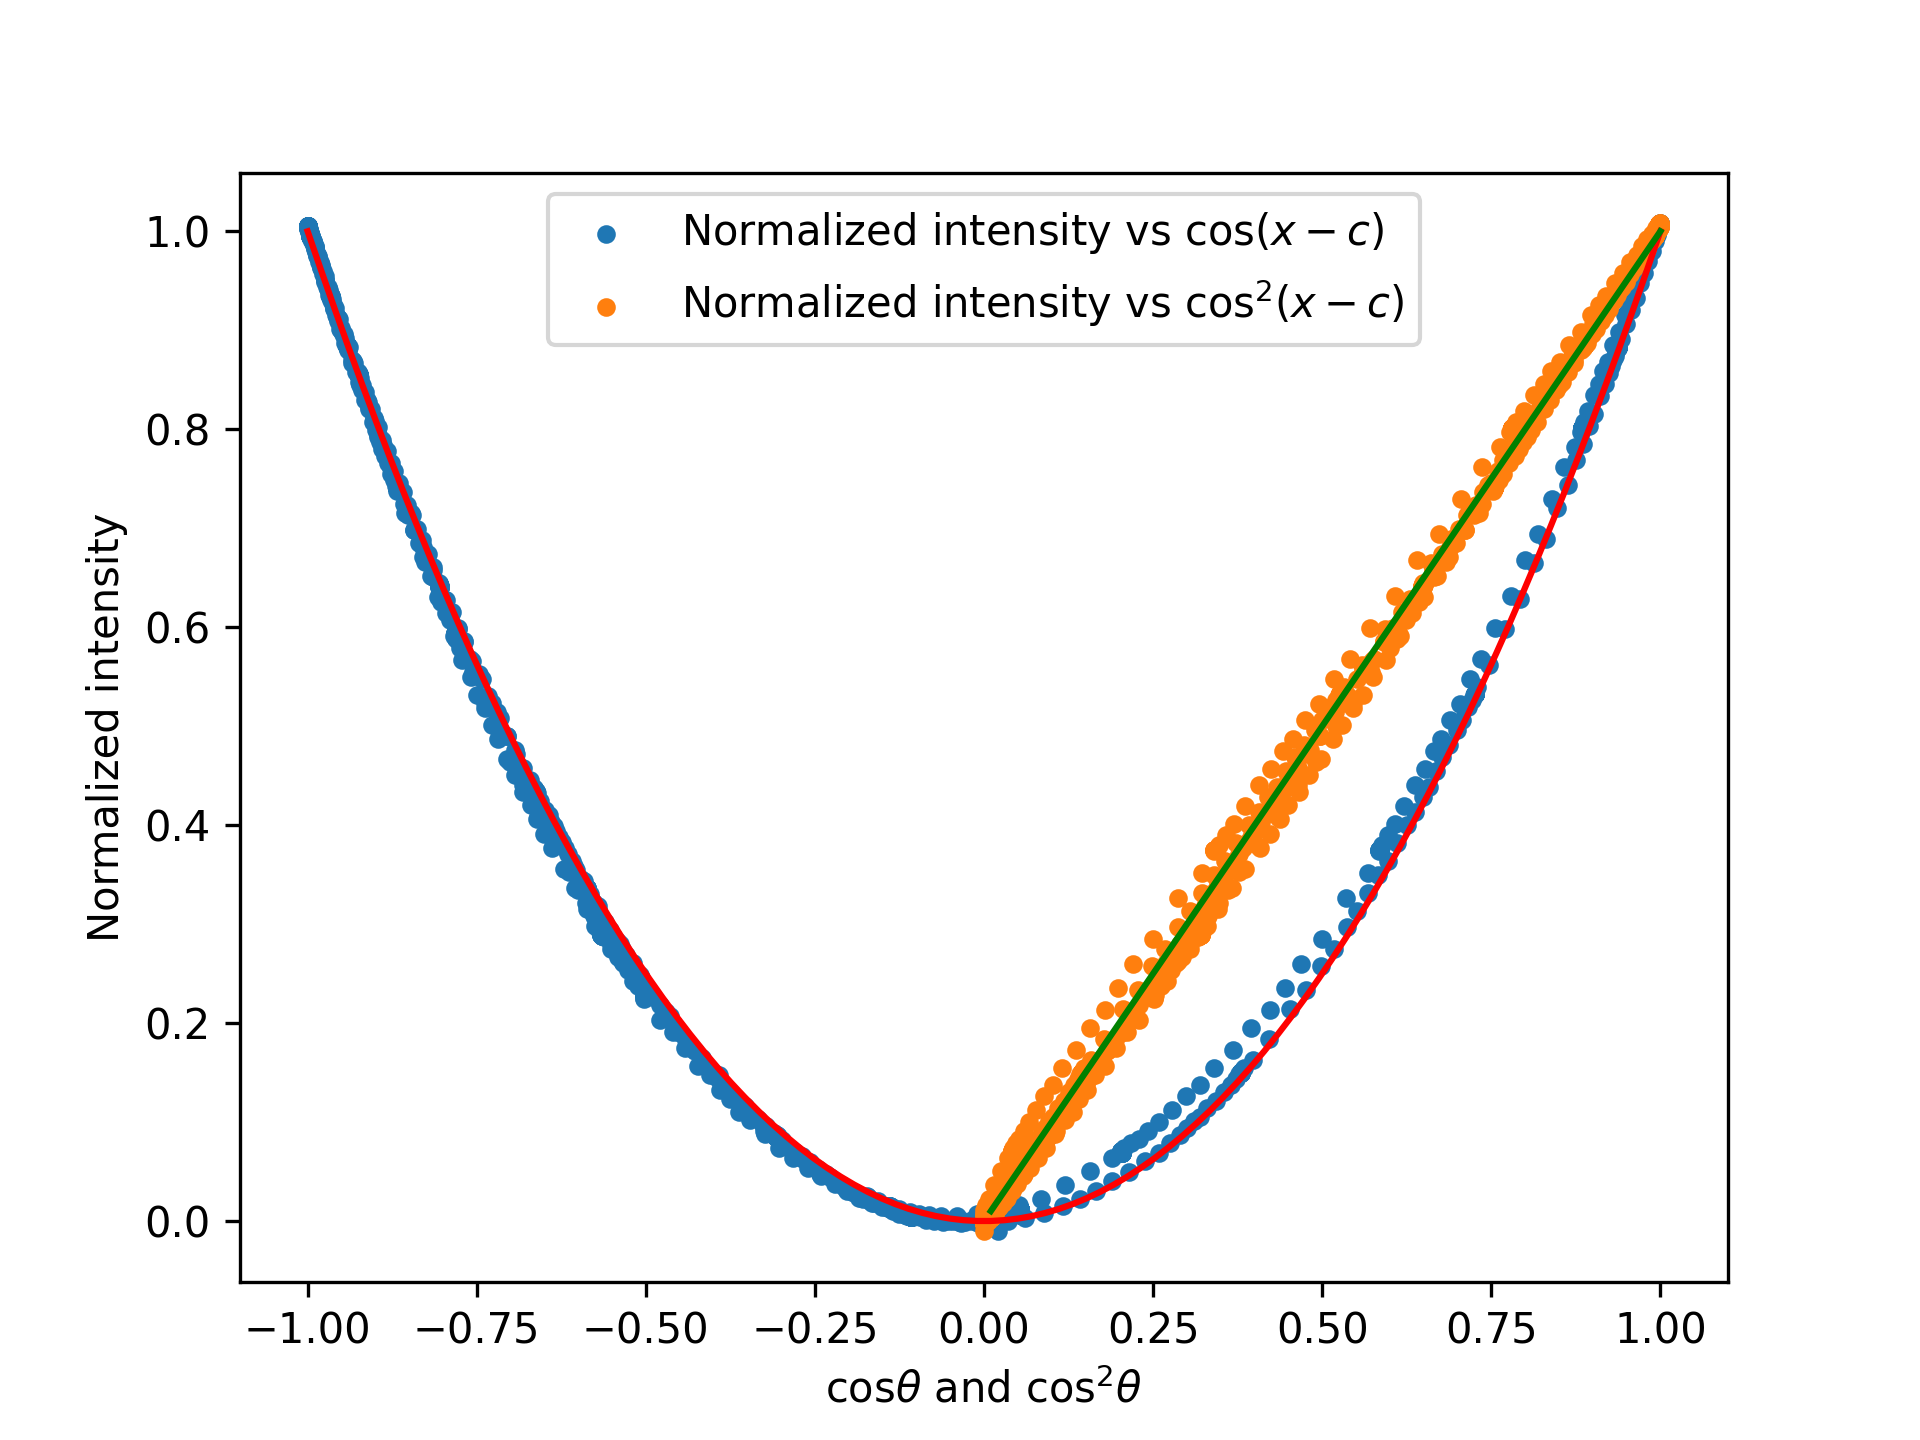
\includegraphics[width=1.1\textwidth]{./pol_1_normal.png}
                \caption{Polariser I}
        \end{subfigure}
        \begin{subfigure}[b]{0.50\textwidth}
                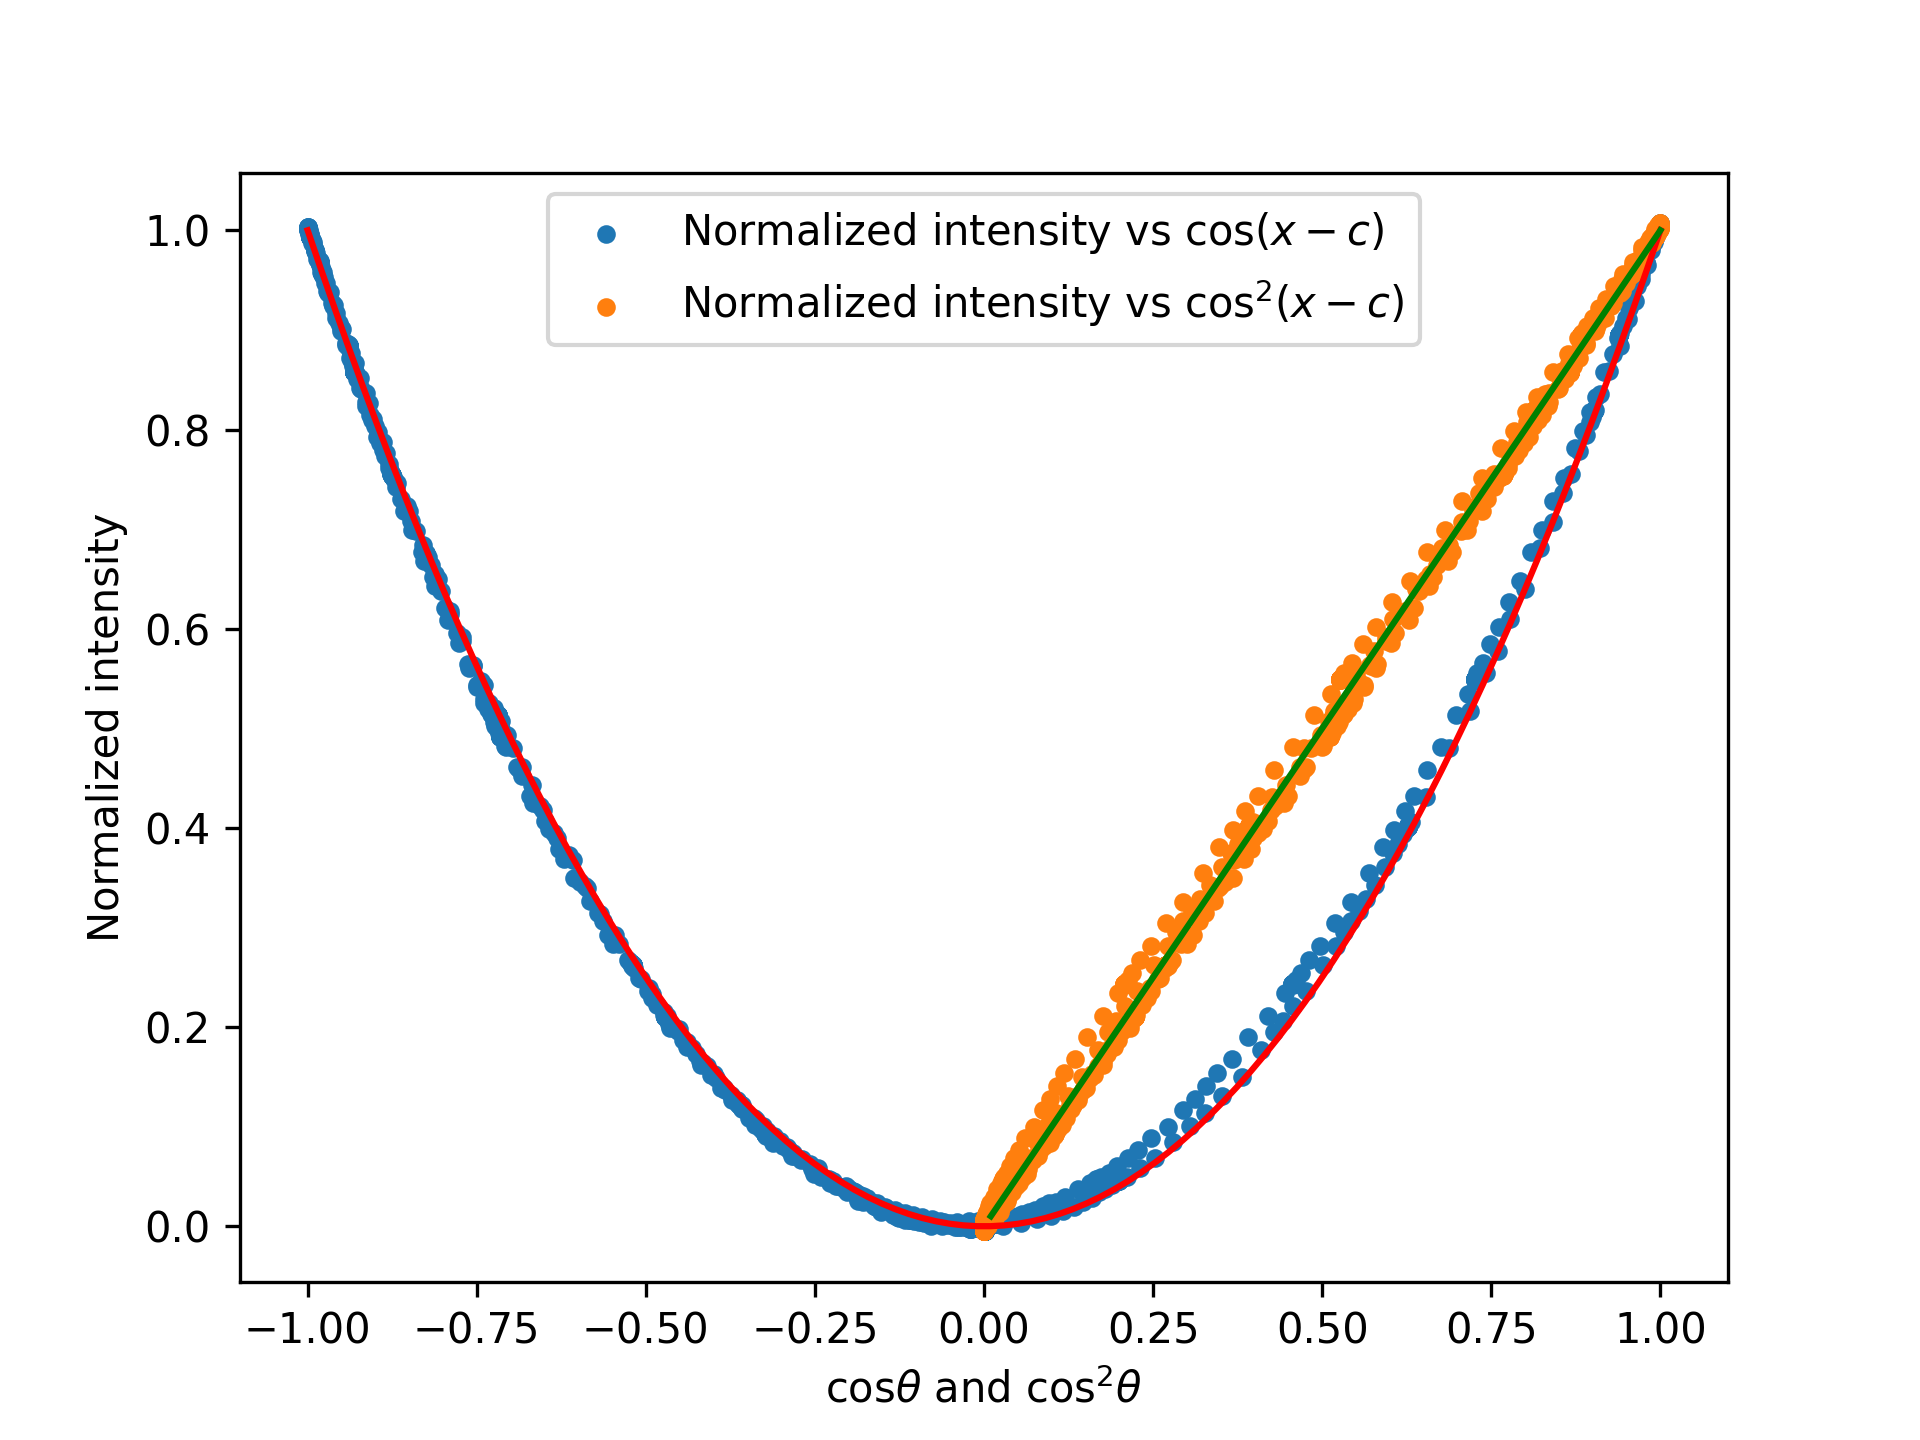
\includegraphics[width=1.1\textwidth]{./pol_2_normal.png}
                \caption{Polariser II}
        \end{subfigure}
        \caption{The intensities from the polariser-analyser setup has been normalised as $I_{normal} = (I - a) / b$.
        These have been plotted against $\cos(x - c)$ and $\cos^2(x - c)$. The curves $y = x^2$ and $y = x$ have been drawn in red and green respectively
        to emphasize the $\cos^2$ relationship.}
        \label{fig:polarisers_normal}
        \end{figure}
        
        The fit parameters and uncertainties from Fig.~\ref{fig:polarisers} are as follows.
        \begin{center}
        \begin{tabular}{l|ccc}
                        &       $a$             & $b$                   & $c$ \\\hline
                Set I   &  $21.95 \pm 0.01$     & $-20.69 \pm 0.02$     & $-7.80 \pm 0.01$ \\
                Set II  &  $21.34 \pm 0.01$     & $-20.13 \pm 0.01$     & $-7.83 \pm 0.01$
        \end{tabular}
        \end{center}

        Because of the manner in which the fit has been made ($b < 0$), we have $I_{max} = a$ and $I_{min} = a + b$. Thus,
        \[
                \mathcal{P} = \frac{I_{max} - I_{min}}{I_{max} + I_{min}} = \frac{a - (a + b)}{a + (a + b)} = \frac{-b}{2a + b}, \qquad
                \mathcal{P}' = 1 - \frac{I_{min}}{I_{max}} = 1 - \frac{a + b}{a} = \frac{-b}{a}.
        \]
        We calculate these for the two sets of data as follows.
        \[
                \mathcal{P}_{I} = 0.891, \qquad \mathcal{P}_{I}' = 0.943,
        \]
        \[
                \mathcal{P}_{II} = 0.893, \qquad \mathcal{P}_{II}' = 0.943.
        \]\\~\\ 
        We estimate the ellipticity of the light from the waveplate using data from Fig.~\ref{fig:waveplates}.
        \begin{center}
        \begin{tabular}{l|ccc}
                        &       $I_{min}$       & $I_{max}$             & $\eta = I_{min} / I_{max}$ \\\hline
                Set I   &  $6.05 \pm 0.1$       & $10.75 \pm 0.1$       & $0.563$ \\
                Set II  &  $6.80 \pm 0.1$       & $9.05 \pm 0.1$        & $0.751$
        \end{tabular}
        \end{center}
        Thus, neither set exhibits circularly polarised light, since $I_{min} / I_{max}$ is not close to unity.
        Indeed, the particular pattern of alternating magnitudes of the maxima and minima cannot be explained by supposing elliptically polarised light.
        The fitting function $I = (a + b\cos(x - c))(d + e\cos(x - f))$ has been conjectured without a theoretical basis.
        
        \begin{figure}[H]
        \begin{subfigure}[b]{0.50\textwidth}
                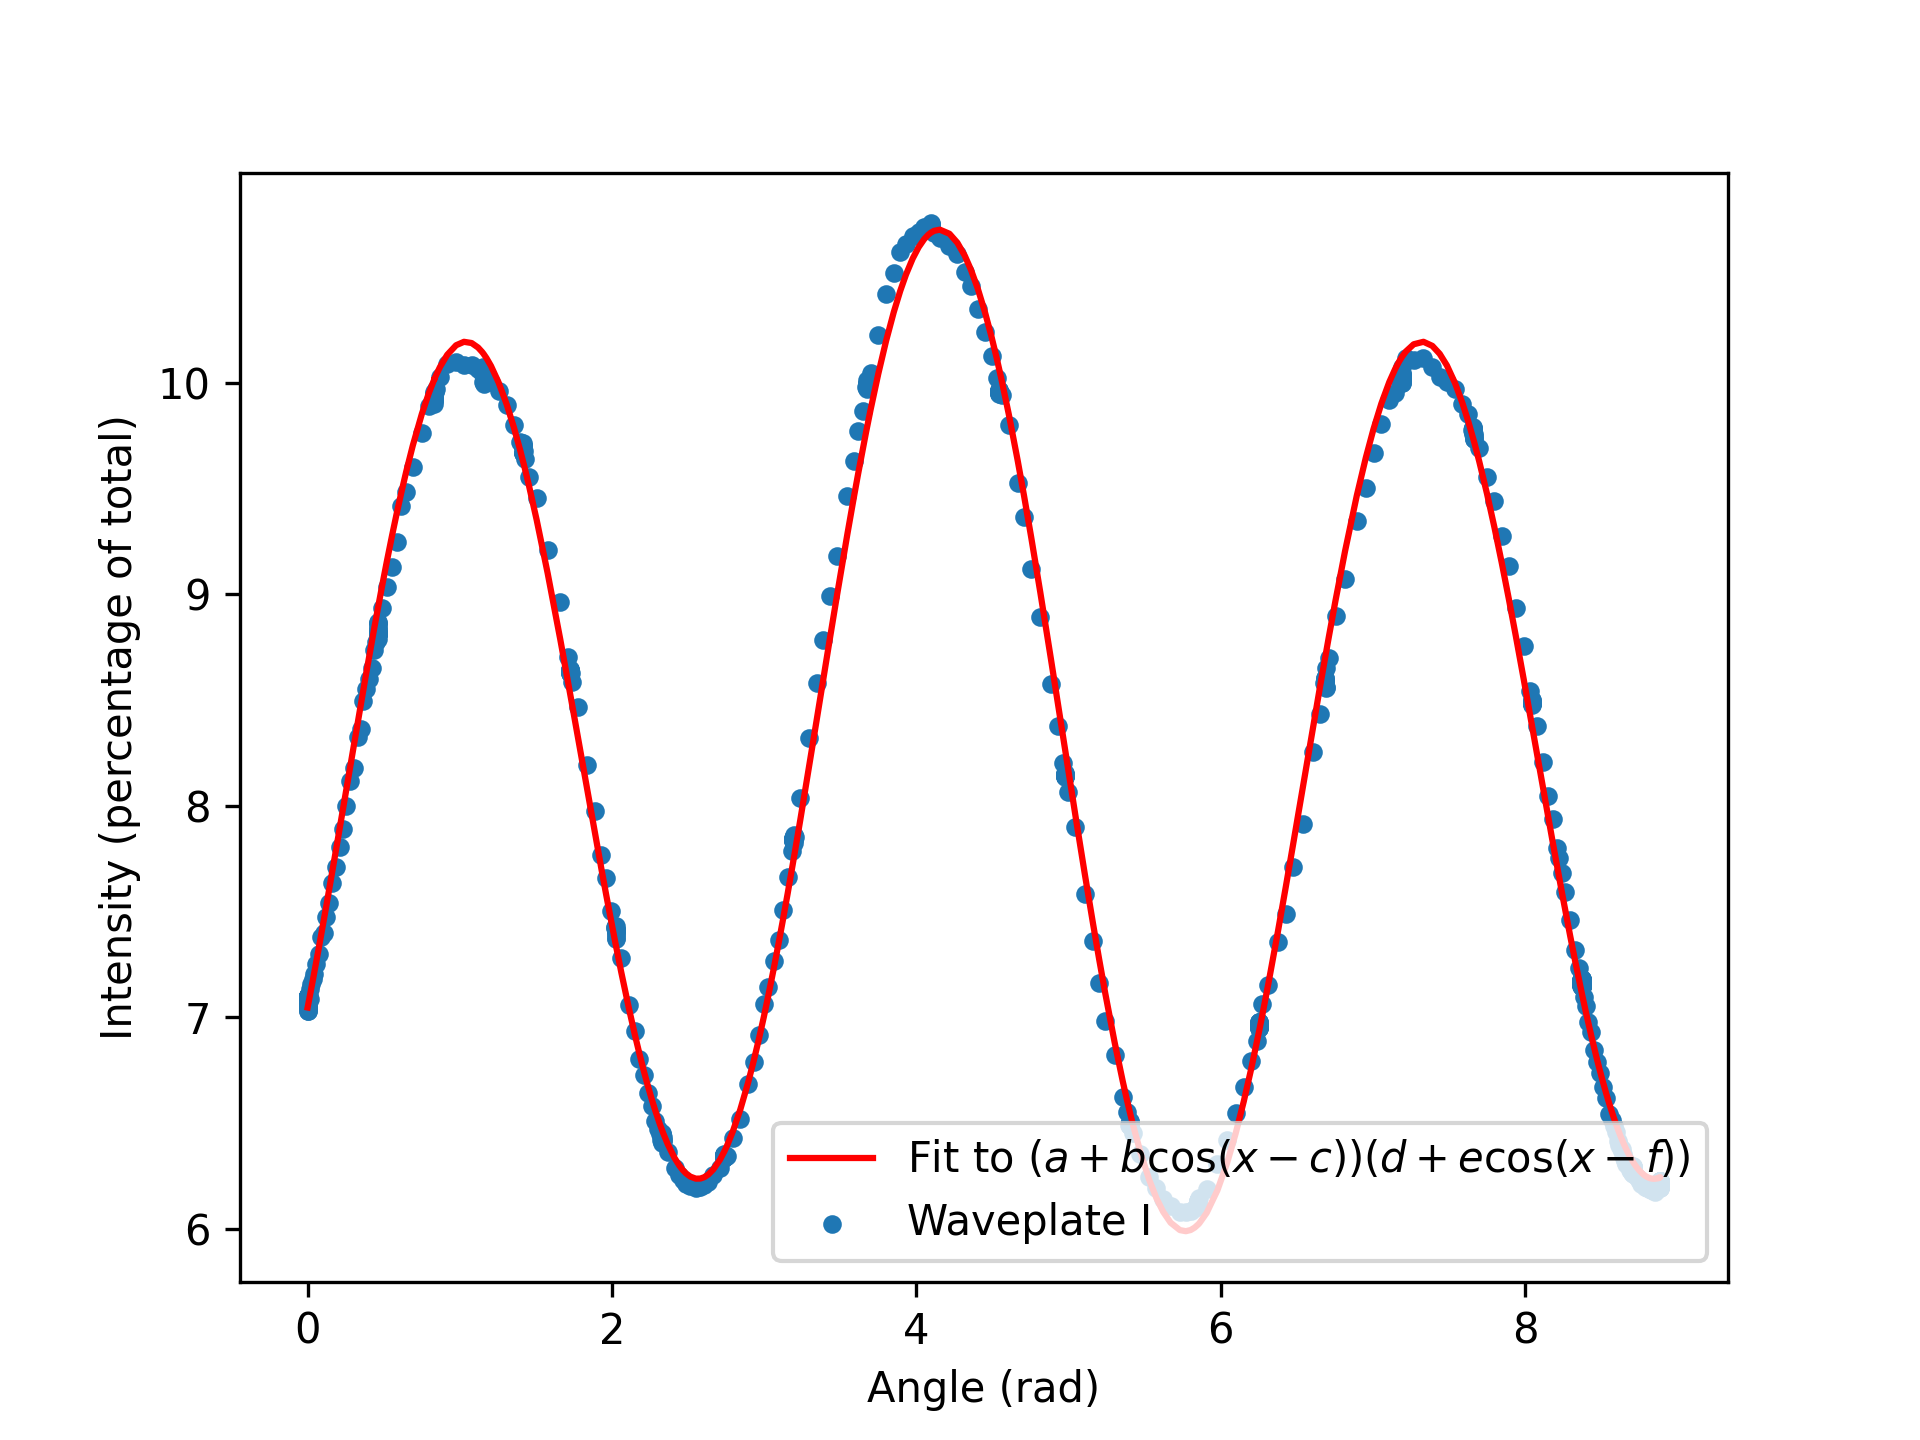
\includegraphics[width=1.1\textwidth]{./wp_1.png}
                \caption{Waveplate I}
        \end{subfigure}
        \begin{subfigure}[b]{0.50\textwidth}
                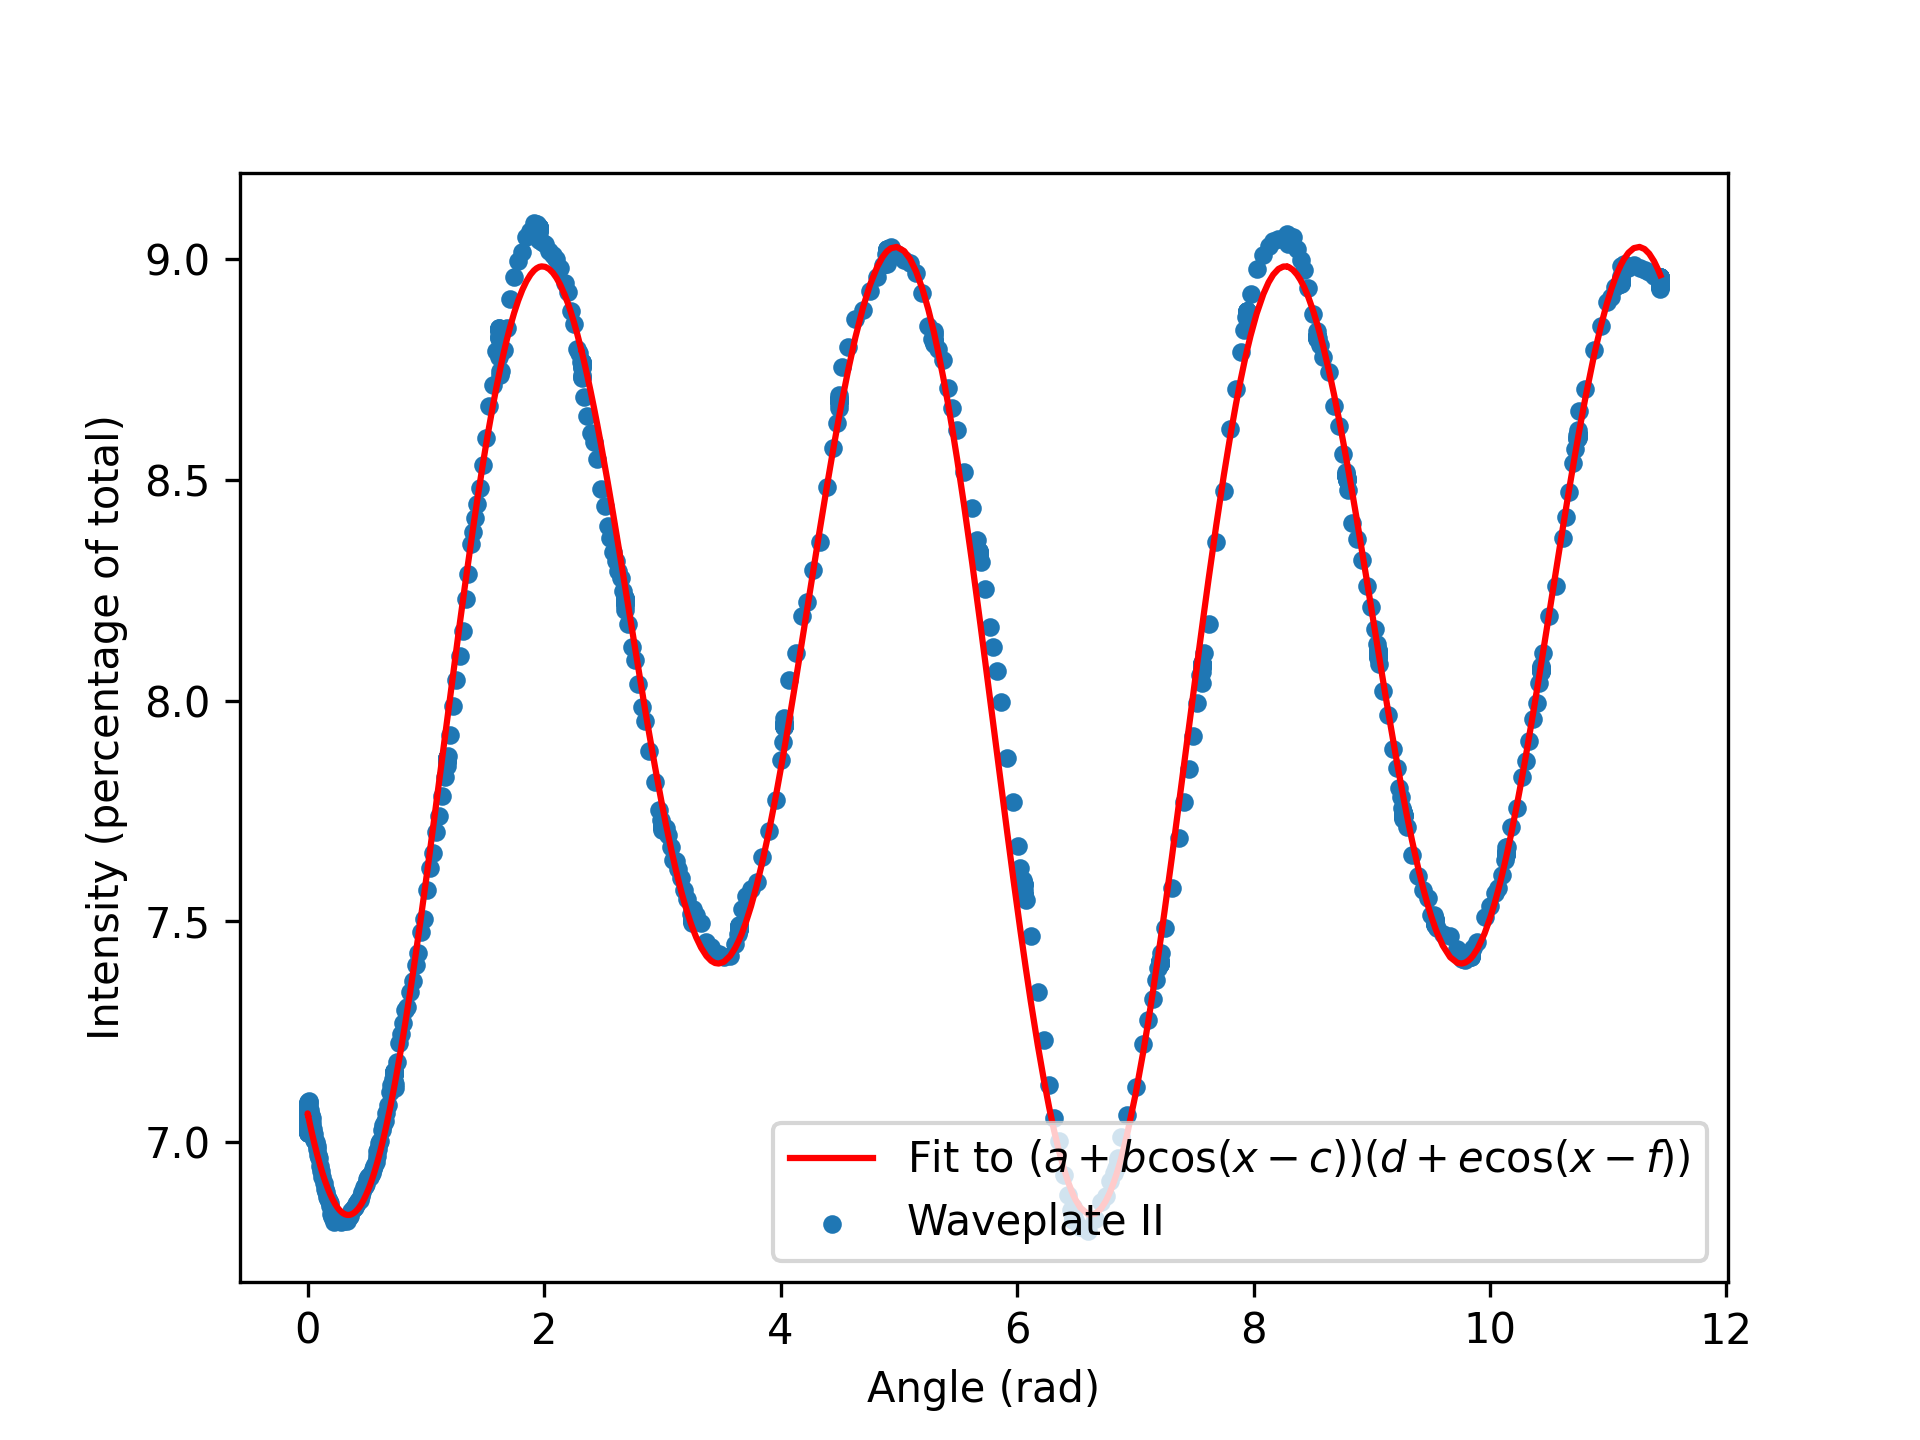
\includegraphics[width=1.1\textwidth]{./wp_2.png}
                \caption{Waveplate II}
        \end{subfigure}
        \caption{Intensities from the waveplate setup as a function of the rotation angle. Note that they do not fit an elliptically polarised light
        distribution, even allowing for imperfect polarisers. Thus, the light from the waveplate is not circularly polarised. The ellipticity is
        estimated as $\eta = I_{min} / I_{max}$.}
        \label{fig:waveplates}
        \end{figure}
        
        \subsection{Error Analysis}
        We write
        \begin{align*}
                (\delta\mathcal{P})^2 &= \left|\pp{\mathcal{P}}{a}\right|^2(\delta a)^2 + \left|\pp{\mathcal{P}}{b}\right|^2(\delta b)^2
                        = \left(\frac{2b}{(2a + b)^2}\right)^2 (\delta a)^2 + \left(\frac{2a}{(2a + b)^2}\right)^2(\delta b)^2, \\
                (\delta\mathcal{P}')^2 &= \left|\pp{\mathcal{P}'}{a}\right|^2(\delta a)^2 + \left|\pp{\mathcal{P}'}{b}\right|^2(\delta b)^2
                        = \left(\frac{b}{a^2}\right)^2 (\delta a)^2 + \left(\frac{1}{a}\right)^2(\delta b)^2, \\
                \left(\frac{\delta \eta}{\eta}\right)^2 &= \left(\frac{\delta I_{min}}{I_{min}}\right)^2 + \left(\frac{\delta I_{max}}{I_{max}}\right)^2.
        \end{align*}
        Thus, we calculate
        \[
                \delta\mathcal{P}_{I} = 0.002, \qquad \delta\mathcal{P}_{I}' = 0.001,
        \]
        \[
                \delta\mathcal{P}_{II} = 0.001, \qquad \delta\mathcal{P}_{II}' = 0.001.
        \]
        \[
                \delta\eta_{I} = 0.011, \qquad \delta\eta_{II} = 0.013.
        \]

        \subsection{Reported Values}
        We see that the degree of polarisation of light produced is $\mathcal{P} = 89.2 \pm 0.2\%$ (or $\mathcal{P}' = 94.3 \pm 0.1\%$, 
        depending on which definition is preferred). 

        We also note that the light produced by the waveplates is not circularly polarised. The measure of ellipticity $\eta$ is not close
        to unity, instead it is $0.563 \pm 0.011$ in the first set and $0.751 \pm 0.013$ in the second.

        \section{Discussion}
        We see that the Malus Law holds very well, and any deviations can be explained by the imperfection of the polariser.
        The degree of polarisation of these polarisers is quite good.

        The behaviour of the polarised light from the waveplate is unexpected, and requires deeper analysis to justify the form
        $(a + b\cos(x - c))(d + e\cos(x - f))$. This is not consistent with elliptically polarised light, and is certainly not with a circular
        polarisation. We may attempt to consider the effects of an imperfect first polariser, or an imperfect waveplate to try and explain
        the form of the intensity curve.

        One hypothesis for the four extrema in the waveplate curve is that the polarisation of the light resembles an off-centre or squashed ellipse.
        The magnitude of a vector from the centre to the edge of such a shape goes through a periodic cycle with two different maxima and
        two minima, much like our intensity distribution. Such a polarisation may have arisen from an imperfect waveplate, perhaps tilted,
        or some external electric field which biases the oscillating vector in some particular direction.
        
        % Suppose that this offset is by a vector $(a, b)$.
        % Thus, the light form the waveplate has $E_x = a + A\cos(\omega t)$, $E_y = b + B\sin(\omega t)$.
        % We assume a perfect polariser rotated by $\theta$, so
        % \begin{align*}
        %         E_\parallel &= (a + A\cos(\omega t))\cos\theta - (b + B\sin(\omega t))\sin\theta, \\
        %         E_\perp     &= (a + A\cos(\omega t))\sin\theta + (b + B\sin(\omega t))\cos\theta.
        % \end{align*}
        % We only let $E_\parallel$ proceed, so we calculate
        % \begin{align*}
        %         E_\parallel^2 &= a^2\cos^2\theta + A^2\cos^2(\omega t)\cos^2\theta + 2aA\cos(\omega t)\cos^2\theta + \\
        %                 &\quad   b^2\sin^2\theta + B^2\sin^2(\omega t)\sin^2\theta + 2bB\sin(\omega t)\sin^2\theta - \\
        %                 &\quad   2\left[ab + aB\sin(\omega t) + bA\cos(\omega t) + AB\cos(\omega t)\sin(\omega t)\right]\cos\theta\sin\theta.
        % \end{align*}
        % Taking time averages, we see that
        % \[
        %         \langle E_\parallel^2 \rangle = a^2\cos^2\theta + \frac{1}{2}A^2\cos^2\theta + b^2\sin^2\theta + \frac{1}{2}B^2\sin^2\theta - 
        %                 2ab\cos\theta\sin\theta.
        % \]
        

        \subsection{Sources of error}
        The imperfections in the polariser comprise a source of systematic error. The least count of the rotary motion sensor introduces
        random error, as does any external lighting.

        \section{Conclusion}
        In conclusion, we have verified the Malus Law and have analysed the effect of waveplates on lieanrly polarised light.

        % \nocite{*}
        % \bibliographystyle{plain}
        % \bibliography{ref}

\end{document}
